% 03-freertos-porting.tex

\section{Part 2 - FreeRTOS Porting}

\begin{frame}{Overview}
    \begin{itemize}
        \item To test the \textbf{FreeRTOS Porting} on \textbf{QEMU}, a very simple application was created.
        \item The application runs a basic task that prints a message every second.
        \item If everything works correctly, it means that the \textbf{FreeRTOS Porting} has been successfully implemented.
    \end{itemize}
\end{frame}

\begin{frame}{Setting Up FreeRTOS}
    \begin{enumerate}
        \item \textbf{Cloning} the FreeRTOS repository.
        \item Creating the directory \textbf{structure}: \texttt{App/} and \texttt{App/Peripherals/}.
        \item Creating and implementing the following files in the \texttt{App/} directory:
            \begin{itemize}
                \item \texttt{s32\_startup.c}, \texttt{s32\_linker.ld}
                \item \texttt{FreeRTOSConfig.h}
                \item \texttt{Makefile}
                \item \texttt{main.c}
                \item \texttt{Peripherals/}: \texttt{uart.c}, \texttt{printf-stdarg.c} with their respective header files
            \end{itemize}
    \end{enumerate}
\end{frame}

\begin{frame}{Setting Up FreeRTOS}
    
    % TODO: is this frame needed ?

\end{frame}

\begin{frame}[fragile]{Running FreeRTOS on QEMU}
    \begin{itemize}
        \item \texttt{main.c}:
            \begin{lstlisting}[language=C]
xTaskCreate(vTask1, "Task1", configMINIMAL_STACK_SIZE, NULL, mainTASK_PRIORITY, NULL);

void vTask1(void *pvParameters) 
{
    (void) pvParameters;

    for (;;) 
    {
        printf("Task1 is running...\n");
        vTaskDelay(1000);
    }
}
            \end{lstlisting}
    \end{itemize}
\end{frame}

\begin{frame}[fragile]{Running FreeRTOS on QEMU}
    \begin{itemize}
        \item Run the \textbf{Test}:
            \begin{itemize}
                \item \texttt{cd App \&\& make run}
            \end{itemize}
    \end{itemize}
    \begin{figure}[h]
        \centering
        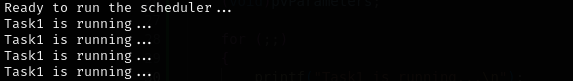
\includegraphics[width=0.75\textwidth]{images/freertos_porting.png}
        \caption{FreeRTOS Porting Test.}
    \end{figure}
\end{frame}
